\chapter{Monovariate Benchmark Datasets}
\label{apd:monovariate_datasets}\index{Monovariate Benchmark Datasets}

The Taiwan Stock Exchange Capitalization Weighted Stock Index (TAIEX)\footnote{\url{http://www.twse.com.tw/en/products/indices/Index_Series.php}. Access in 23/05/2016} is a well known economic time series data commonly used in the FTS literature. This dataset is sampled from 1995 to 2014 time window, and has the averaged daily index by business day. This is a stationary time series dataset whose Augmented Dickey-Fuller (ADF) statistic is $-2.65$ where the critical value for $\alpha = 0.05$ is $-2.86$.
\index{Taiwan Stock Exchange Capitalization Weighted Stock Index}\index{TAIEX}


The National Association of Securities Dealers Automated Quotations -  Composite Index (NASDAQ \^IXIC)\footnote{\url{http://www.nasdaq.com/aspx/flashquotes.aspx?symbol=IXIC\&selected=IXIC}. Access in 23/05/2016} is an economical index already used in the FTS literature . The historical data was sampled from 2000 to 2016 time window, and has the averaged daily index by business day. This is a stationary time series dataset whose ADF statistic is $0.04$ where the critical value for $\alpha = 0.05$ is $-2.86$.
\index{National Association of Securities Dealers Automated Quotations}\index{NASDAQ}

The S\&P500 - Standard \& Poor's 500 \footnote{\url{https://finance.yahoo.com/quote/\%5EGSPC/history?p=\%5EGSPC}. Access in 19/03/2017} is a market index composed by 500 assets quoted on New York Stock Exchange and Nasdaq. This dataset contains the averaged daily index, by business day, from 1950 to 2017 with 16000 instances. This is a stationary dataset whose ADF Statistic is 0.00 where critical value for $\alpha = 0.05$ is $-2.86$.
\index{Standard \& Poor's 500}\index{S\&P 500}

In order to contribute with the research reproducibility, all data and source codes are available in the following URL \url{http://bit.ly/scalable_probabilistic_fts_appendixA}.
\index{Reproducibility}\index{Source codes}

\begin{figure}
    \centering
    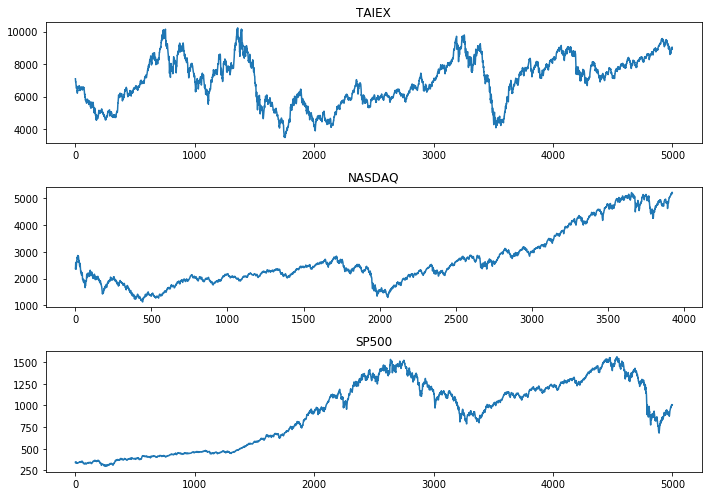
\includegraphics[width=\textwidth]{figures/datasets.png}
    \caption{Benchmark datasets}
    \label{fig:datasets}
\end{figure}

\begin{figure}
    \centering
    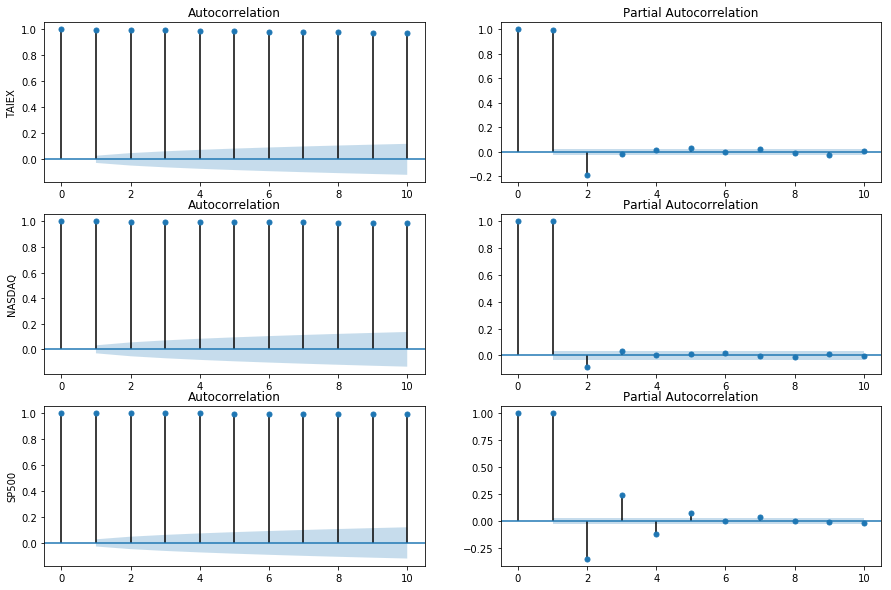
\includegraphics[width=\textwidth]{figures/datasets_acf.png}
    \caption{Autocorrelation and Partial Autocorrelation plots for each benchmark dataset}
    \label{fig:datasets_acf}
\end{figure}

